\newpage

\section{Wyniki badań}

Pierwsze pomiary widma ramanowskiego zostały wykonane dla kryształku $\mathbf{Ga_2S_3}$ na podłożu $\mathbf{GaP}$. W uzyskanym widmie ramanowskim widać zarówno piki pochodzące od kryształku $\mathbf{Ga_2S_3}$ oraz pochodzące od podłoża, rysunek 26.

\begin{figure}[H]
	\begin{center}
		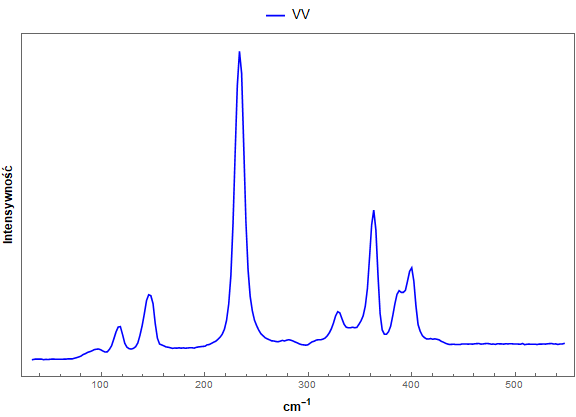
\includegraphics[width=0.8\linewidth]{Wyniki/Raman/plotGapWithGa2S3.png}
		\caption{Widmo ramanowskie dla monokryształku  $\mathbf{Ga_{2}S_{3}}$ na podłożu $\mathbf{GaP}.$}
	\end{center}
\end{figure}

Piki oznaczone numerami 1,2,3,4,6 odpowiadają widmu ramanowskiemu dla $\mathbf{Ga_{2}S_{3}}$, a piki 5,7 odpowiadają widmu ramanowskiemu dla podłoża $\mathbf{GaP}$. Piki pochodzące od $\mathbf{GaP}$ znacznie utrudniają analizę piku 4 i 6. A poza tym można przypuszczać, że nie wszystkie piki, odpowiadające $\mathbf{Ga_{2}S_{3}}$ są widoczne z powodu obecności pików o numerach 5 i 7. 

Pomiary dla $\mathbf{Ga_{2}S_{3}/GaP}$ zostały zrobione tylko w konfiguracji VV dlatego, że później postanowiono przenieść kryształki na inną powierzchnię (szklaną) aby pozbyć się niepożądanych pików na widmie ramanowskim. 

Aby odseparować widma ramanowskie dla $\mathbf{Ga_{2}S_{3}}$ i $\mathbf{GaP}$ wyknone zostały pomiary ramanowskie dla czystej płytki podłożowej $\mathbf{GaP}$, rysunek 27. Żeby to potwierdzić zostało uzyskane widmo ramanowskie dla $\mathbf{GaP}$, które pokazano na rysunku poniżej:

\begin{figure}[H]
	\begin{center}
		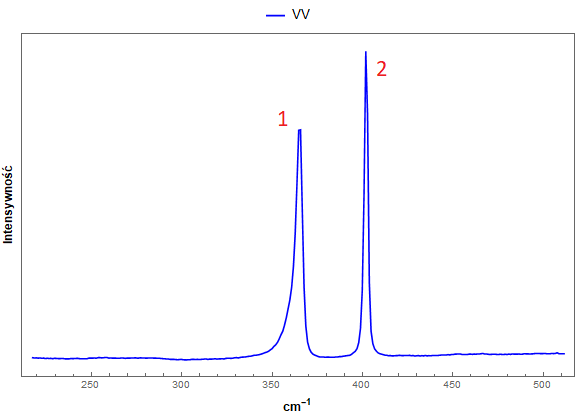
\includegraphics[width=0.8\linewidth]{Wyniki/Raman/plotGaP.png}
		\caption{Widmo ramanowskie dla pików $\mathbf{GaP}$. Widoczne są dwa wyraźne piki: 1 - dla około 360 cm$^{-1}$, 2 - dla około 400 cm$^{-1}$.}
	\end{center}
\end{figure}

Przy opracowywaniu wyników pomiarowych dla polaryzacji VV wykonane zostały wykresy polaryzacyjne dla pików oznaczonych numerem 1 i 2 dla $\mathbf{GaP}$. Wykresy te są przedstawione na rysunku 28. Widmo polaryzacyjne w konfiguracji VV dla kryształku $\mathbf{Ga_2S_3}$ na podłożu $\mathbf{GaP}$ nie zostały przedstawione w tej pracy ponieważ lepszej jakości widma zostały uzyskane dla kryształku $\mathbf{Ga_2S_3}$ przeniesionych na podłoże szklane.
\begin{figure}[H]
	\begin{minipage}[h]{0.5\linewidth}
		\center{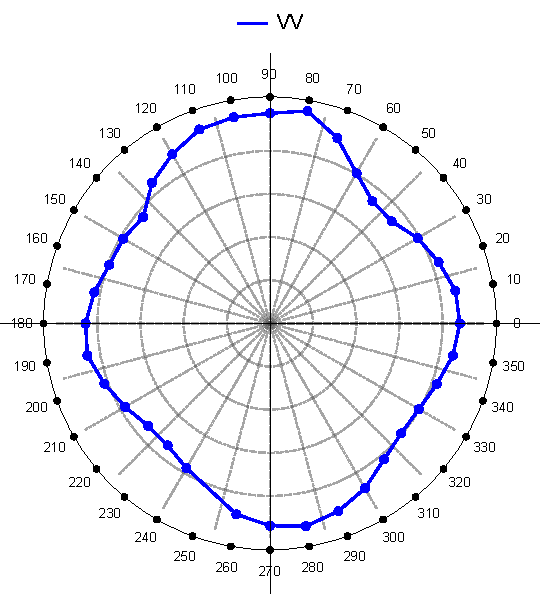
\includegraphics[width=0.8\linewidth]{Wyniki/WidmoPolaryzacyjne/plot5GaP.pdf}} \\ a) 
	\end{minipage}
	\hfill
	\begin{minipage}[h]{0.5\linewidth}
		\center{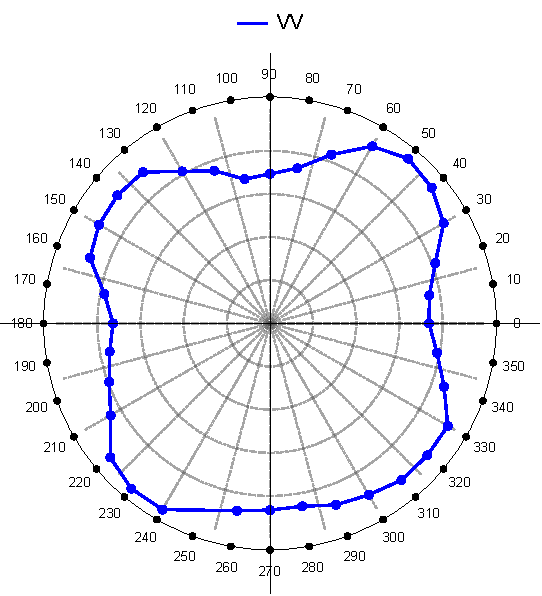
\includegraphics[width=0.8\linewidth]{Wyniki/WidmoPolaryzacyjne/plot7GaP.pdf}} \\b)
	\end{minipage}
	\caption{Widmo polaryzacyjne w konfiguracji VV dla pikow ramanowskich GaP. a) odpowiada pikowi 1 - około 360 cm-1, b) odpowiada 2) - około 400cm-1}
\end{figure}

W dalszej części pracy zostały wykonane pomiary ramanowskie dla kryształków Ga2S3 przeniesionych na płytkę szklaną. Na rysunku 29 zostało przedstawione przykładowe widmo ramanowskie w konfiguracji VV i VH dla takiego kryształku.

\begin{figure}[H]
	\begin{center}
		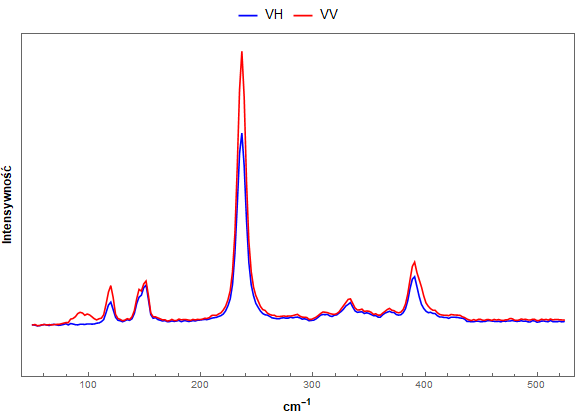
\includegraphics[width=0.8\linewidth]{Wyniki/Raman/plotVVandVH.png}
		\caption{Widmo ramanowskie dla kryształku $\mathbf{Ga_{2}S_{3}}$ na płytce szklanej wykonanej dla konfiguracji VV i VH.}
	\end{center}
\end{figure}

Na powyższym widmie ramanowskim zostało wyróżnionych 7 pików. 1 $\rightarrow$ 117$cm^{-1}$, 2 $\rightarrow$ 143$cm^{-1}$, 3 $\rightarrow$ 149$cm^{-1}$, 4 $\rightarrow$ 235$cm^{-1}$, 5 $\rightarrow$ 309$cm^{-1}$, 6 $\rightarrow$ 330$cm^{-1}$, 7 $\rightarrow$ 390$cm^{-1}$. Dzięki eliminacji podłoża GaP uzyskano większą rozdzielczość w widmie ramanowskim Ga2S3. Ewolucję widma ramanowskiego Ga2S3 konfiguracji VV dla roznych kątów polaryzacji przedstawiono na rysunku 30.

\begin{figure}[H]
	\begin{center}
		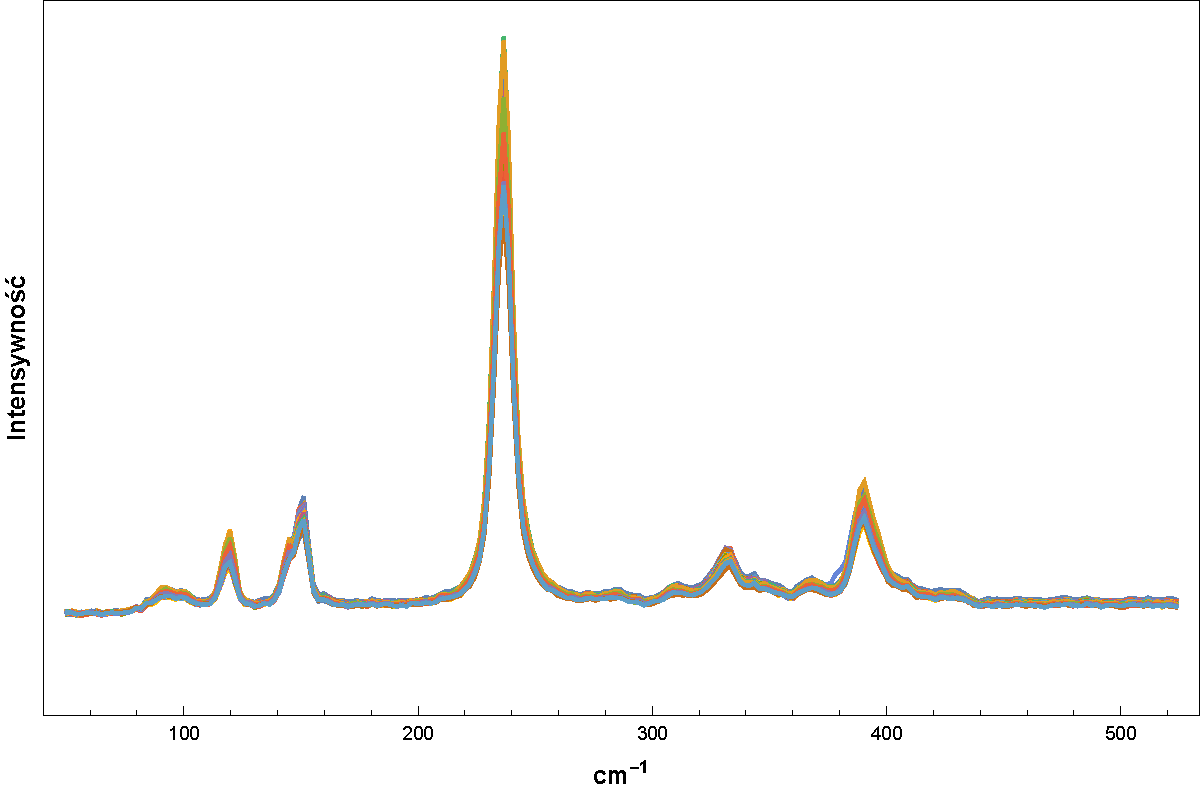
\includegraphics[width=0.8\linewidth]{Wyniki/Raman/plotAllVV.pdf}
		\caption{Widma ramanowskie dla 36 różnych kątów polaryzacji (z krokiem co 5 stopni) dla konfiguracji VV.}
	\end{center}
\end{figure}

Dla każdego piku na widmie ramanowskim zostało uzyskane 36 punktów na widmie polaryzacyjnym, obracając co 5 stopni polaryzacją ($"$półfalówką$"$). Dla pików 1,4,7 została dopasowana pojedyncza funkcja Voigt'a\footnote{Jest mieszaną funkcją: Gauss + Lorentz}. Dla pików 2 i 3 oraz 5 i 6 została dopasowana podwójna funkcja Voigt'a. Uzyskane w wyniku dopasowania pole pod krzywą piku odpowiada natężeniu danego piku ramanowskiego. Na wykresie Arrheniusa naniesione zostały znormalizowane wartości natężeń pików w funkcji konta polaryzacji. Na poniższych rysunkach zostały przedstawione zależności polaryzacyjne dla pików 1-7 dla $\mathbf{Ga_{2}S_{3}}$.

\begin{figure}[H]
	\begin{center}
		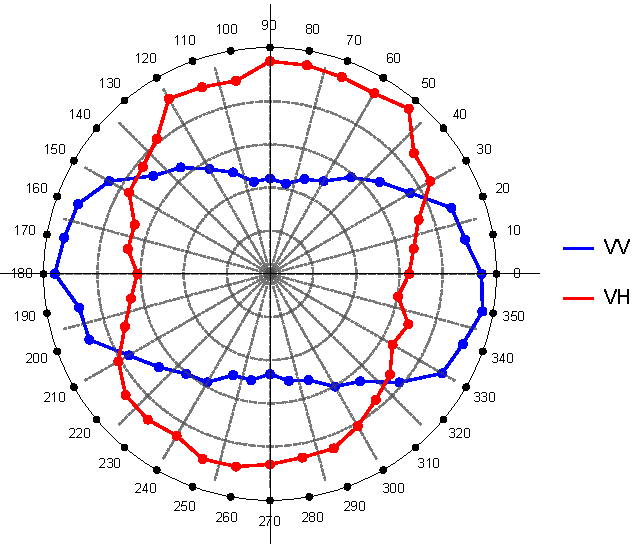
\includegraphics[width=0.75\linewidth]{Wyniki/WidmoPolaryzacyjne/plot117.pdf}
		\caption{Widmo polaryzacyjne dla pika 1 $\rightarrow$ 117$cm^{-1}$ }
	\end{center}
\end{figure}

\begin{figure}[H]
	\begin{center}
		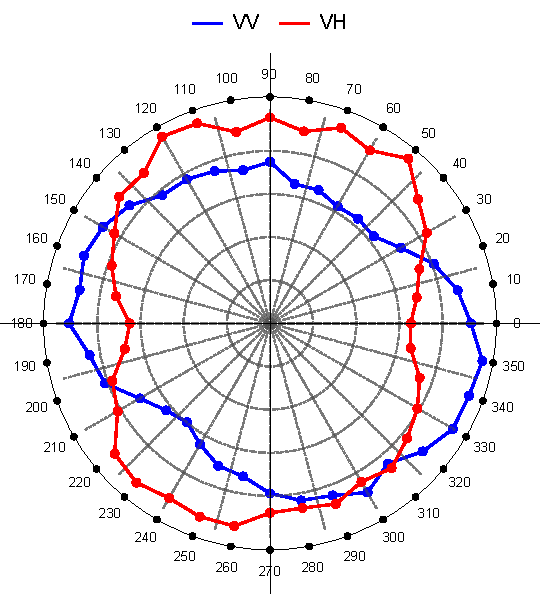
\includegraphics[width=0.75\linewidth]{Wyniki/WidmoPolaryzacyjne/plot143.pdf}
		\caption{Widmo polaryzacyjne dla pika 2 $\rightarrow$ 143$cm^{-1}$ }
	\end{center}
\end{figure}

\begin{figure}[H]
	\begin{center}
		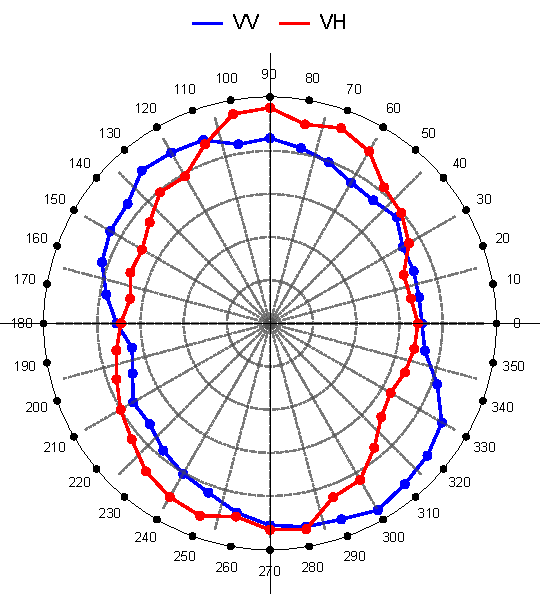
\includegraphics[width=0.75\linewidth]{Wyniki/WidmoPolaryzacyjne/plot149.pdf}
		\caption{Widmo polaryzacyjne dla pika 3 $\rightarrow$ 149$cm^{-1}$ }
	\end{center}
\end{figure}

\begin{figure}[H]
	\begin{center}
		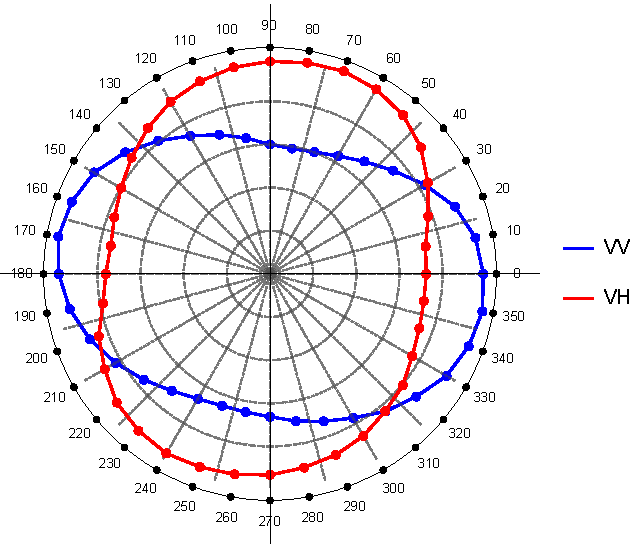
\includegraphics[width=0.75\linewidth]{Wyniki/WidmoPolaryzacyjne/plot235.pdf}
		\caption{Widmo polaryzacyjne dla pika 4 $\rightarrow$ 235$cm^{-1}$ }
	\end{center}
\end{figure}

\begin{figure}[H]
	\begin{center}
		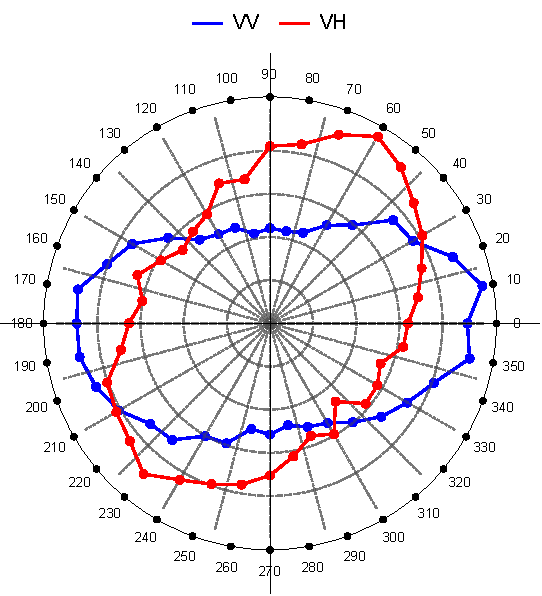
\includegraphics[width=0.75\linewidth]{Wyniki/WidmoPolaryzacyjne/plot309.pdf}
		\caption{Widmo polaryzacyjne dla pika 5 $\rightarrow$ 309$cm^{-1}$ }
	\end{center}
\end{figure}

\begin{figure}[H]
	\begin{center}
		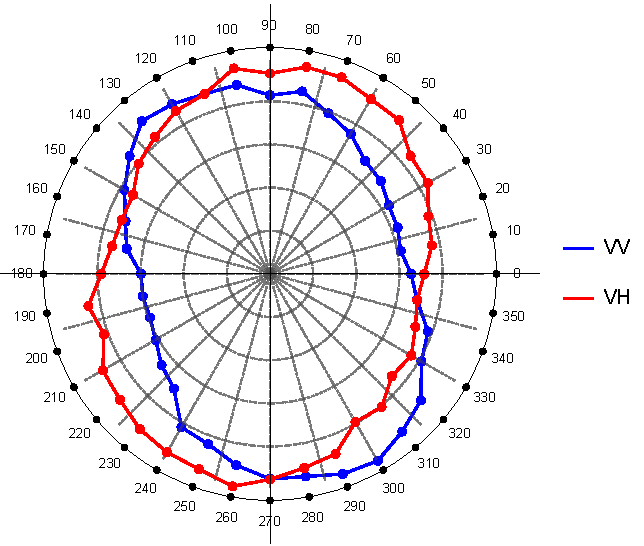
\includegraphics[width=0.75\linewidth]{Wyniki/WidmoPolaryzacyjne/plot330.pdf}
		\caption{Widmo polaryzacyjne dla pika 6 $\rightarrow$ 330$cm^{-1}$ }
	\end{center}
\end{figure}

\begin{figure}[H]
	\begin{center}
		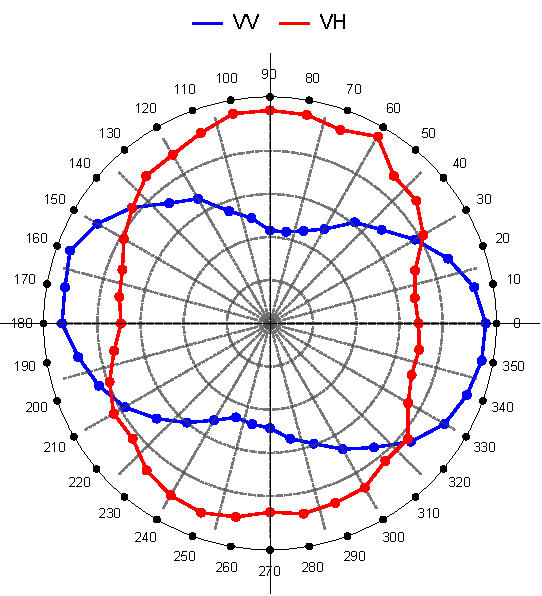
\includegraphics[width=0.75\linewidth]{Wyniki/WidmoPolaryzacyjne/plot390.pdf}
		\caption{Widmo polaryzacyjne dla pika 7 $\rightarrow$ 390$cm^{-1}$ }
	\end{center}
\end{figure}

Jakość dopasowania krzywej Voigt'a do piku ramanowskiego była związana z natężeniem piku, dla większych pików jest mniejszy bląd. Niemniej jednak uzyskalem regularne krzywe polaryzacyjne które posiadały dwa wyraźne maksima w zakresie od 0 do 360 stopni. Krzywe polaryzacyjne analizowane w dalszej części pracy.
